\documentclass[11pt]{article}
\usepackage[margin=1in]{geometry}
\usepackage[T1]{fontenc}
\usepackage{graphicx,amsmath,amssymb,booktabs,array,url,hyperref}
\providecommand{\doi}[1]{\href{https://doi.org/\detokenize{#1}}{\url{https://doi.org/#1}}}
\let\citep\cite
\let\citet\cite
\providecommand{\tightlist}{\setlength{\itemsep}{0pt}\setlength{\parskip}{0pt}}
\title{Cortex AI: Permission-Gated Temporal Retrieval and
Authority-Aware Conflict Abstention for Enterprise Policy Knowledge}
\author{Aditya Gholap \and Arya Dhumal \and Ashwin Gudur \and Yashraj
Bansal}
\date{}
\emergencystretch=1.5em
\begin{document}
\maketitle
\begin{center}\small Department of Computer Science and Engineering, MIT
School of Computing, MIT Art, Design and Technology University, Pune,
India\\{[}Corresponding author and email to be confirmed{]}\end{center}
\begin{abstract}
An enterprise policy answer must use evidence the requester can read and
that applies on the requested date. Cortex AI evaluates reviewed numeric
claims under tenant-scoped document grants and effective-date
constraints. A lexical hit triggers expansion of authorized peers,
allowing the decision rule to detect incompatible values at the highest
authority tier. The strict path verifies cited text before returning a
value, and an unresolved conflict causes abstention unless a verified
Auditor choice applies to the same evidence. The development fixture
reproduced 12 of 12 expected outcomes, 15 of 15 labeled eligible
policy-question pairs, and 10 of 10 exact citation span and hash checks.
On a second fictional corpus, the full service matched the labeled
outcomes and source sets for all 16 questions. A publication-recency
comparator matched 5 questions and each valid-time comparator matched
14. Both valid-time comparators committed to an answer on two questions
about one unresolved policy dispute. The results describe designed cases
and the monitored application stages.
\end{abstract}
\noindent\textbf{Keywords.} enterprise policy retrieval, access control,
valid time, conflict abstention, evidence provenance
\section{Introduction}\label{introduction}

Consider an employee trying to find their annual-leave entitlement. A
search may return an older policy, the version currently in force, and a
revision that has been approved but is not yet effective. All three can
contain the same keywords, yet only one may apply to the requested date.
A different problem arises when two applicable policies disagree: citing
one of them would conceal the uncertainty. The employee's access rights
matter as well, because a policy administrator may see records that the
employee is not permitted to read.

Knowledge-management research documents organizational barriers to
finding and using internal knowledge \citep{alavi}. Retrieval-augmented
generation shows how retrieved documents can ground open-domain answers
\citep{lewis}. Policy answering adds a decision about which sources are
admissible and which claims govern. A genuine citation to a
future-effective edition or to only one of two competing sources can
still support the wrong decision.

Cortex AI addresses this narrower policy-decision problem for four
reviewed numeric topics: annual leave, remote work, notice period, and
executive bonus. Before producing an answer, it enforces tenant and
document access, evaluates approved scope and effective dates, expands
the eligible set of comparable claims, and checks authority and
disagreement. A supported value is accompanied by an exact source span;
an unresolved conflict instead leads to abstention. An Auditor can also
record a verifiable resolution for a specific conflict. None of these
mechanisms is novel in isolation. What we evaluate is the behavior of
their combined, inspectable implementation, from the admissible evidence
set to the final answer or abstention.

We reran the development checks and tested the same pipeline on a second
fictional corpus. The study defined the applicability and disagreement
labels before execution with Codex assistance. The new labels await
independent adjudication. A separate experiment examines related-passage
retrieval because it does not determine which claim governs.

\section{Related Work}\label{related-work}

\subsection{Enterprise authorization and lexical
retrieval}\label{enterprise-authorization-and-lexical-retrieval}

The NIST role-based access control model formalizes the relationship
among users, roles and permissions \citep{sandhu}. Cortex uses roles for
action permissions and document grants for resource visibility.
B\"{u}ttcher and Clarke studied access-aware full-text search over a
shared filesystem index and showed that simple postprocessing can expose
information about hidden files \citep{buettcher}. Their work motivates a
careful distinction between database index access and the text or
ranking statistics available to an application stage. Cortex's shared
full-text index stays inside its trusted database. Query eligibility
constrains which IDs are returned, and application ranking is computed
on admitted records. The experiments observe application boundaries and
do not establish the filesystem study's broader security properties.

BM25 formalizes probabilistic lexical ranking \citep{robertson}. BEIR
compares lexical and learned rankings across heterogeneous retrieval
tasks \citep{thakur}. Dense Passage Retrieval shows how learned
representations retrieve passages that need not share surface terms with
the question \citep{karpukhin}. Reciprocal rank fusion combines ranked
lists without requiring scores on a common scale \citep{cormack}. These
works motivate testing lexical and semantic passage recall
independently. They do not prescribe whether a current policy may
override another policy or authorize text retrieval for a given reader.

\subsection{Valid time, contradiction and
support}\label{valid-time-contradiction-and-support}

Time-aware models condition answers on changing facts \citep{dhingra}.
HoH examines coexistence of stale and current information in
retrieval-augmented answering \citep{ouyang}. Re3 uses relevance and
recency with conflict-aware temporal filtering \citep{cao}. TimelyRAG
reranks passages by clause-level validity in evolving documents
\citep{nam}. Cortex takes an effective interval from reviewed metadata
and accepts a requested past, current or future date. Publication
recency is a useful comparator because it implements a different notion
of precedence.

MultiNLI studies entailment, neutrality and contradiction in sentence
pairs \citep{williams}. Ragability evaluates language models given
conflicting and consistent contexts \citep{gross}. Cortex uses a
narrower decision rule: differing normalized integers within the same
policy claim key and strongest authority tier. That restriction allows a
deterministic test of the rule. It also excludes linguistic exceptions,
modality shifts outside the schema and contradictions spread over
several clauses. Selective classification supplies the concepts of risk
and coverage \citep{geifman}. Here, answer coverage can be counted
directly and abstention is triggered by explicit rules, including
missing evidence and unresolved equal-tier disagreement.

ALCE separates citation support from completeness \citep{gao}. RAGAs
separates retrieval and answer quality \citep{es}, and Self-RAG learns
when to retrieve and critique \citep{asai}. For its strict answers,
Cortex verifies the stored span, digest and numeric occurrence before
rendering a fixed sentence. Human review remains responsible for
interpretation. Corpus poisoning research motivates controlling which
versions become eligible \citep{zou}. The effectiveness of review
against malicious approved content remains untested.

\section{Problem Definition and Research
Questions}\label{problem-definition-and-research-questions}

After authentication and routing, we represent a strict policy request
as \(q=(u,t,s,k)\), where \(u\) is the user, \(t\) is the as-of date,
\(s\) is the requested jurisdiction and population, and \(k\) is the
inferred topic. The notation assumes the supported default condition.
Each topic specifies an expected predicate and unit. A reviewed claim
records a normalized value, its document version and extracted-text
span, applicability metadata, and an authority rank. The service can
return a cited value, abstain with a reason, or request clarification.
An unresolved conflict can include citations to competing claims.

\textbf{RQ1.} How does effective-date filtering change selection
relative to publication recency when approval and scope are held fixed?
\textbf{RQ2.} Does strongest-tier abstention avoid choosing a value in
the labeled conflict cases while allowing consistent revisions and
concurrent equivalent claims? \textbf{RQ3.} Do the fixture's restricted
markers reach the observed reasoning, answerer or response stages, and
do the tested direct reads succeed? \textbf{RQ4.} Do returned citation
offsets and digests match the extracted text for the identified source
version? \textbf{RQ5.} Which designated passages appear with the
optional local encoder, and how do warm request times differ?

\section{System Architecture and Trust
Model}\label{system-architecture-and-trust-model}

Figure 1 shows the principal data flows. The browser sends requests to a
FastAPI service. The service derives identity from an opaque session and
checks tenant-local actions before processing protected endpoints. The
authorization predicate for a document requires a same-tenant,
unarchived record and a current direct user or role READ grant. Role
membership determines allowed actions, and administrating a document
workflow does not by itself authorize reading any document in the
tenant.

\begin{figure}
\centering
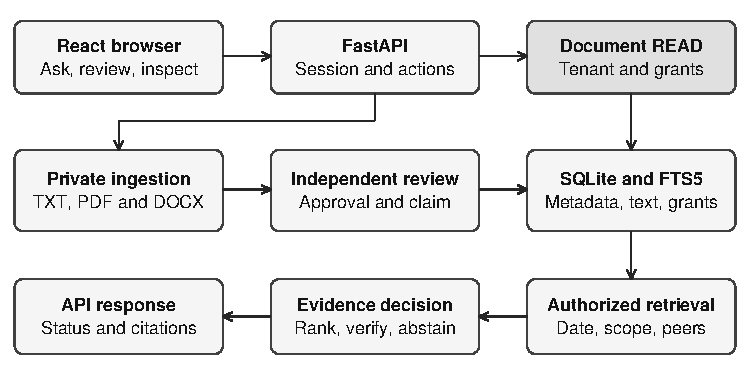
\includegraphics[width=0.89\linewidth,height=\textheight,keepaspectratio,alt={System
architecture. Browser and API actions connect to tenant and document
checks, ingestion, independent review, the evidence store, retrieval,
and answer rendering.}]{../figures/rendered/fig1.pdf}
\caption{System architecture. Browser and API actions connect to tenant
and document checks, ingestion, independent review, the evidence store,
retrieval, and answer rendering.}\label{fig:architecture}
\end{figure}

Access is divided among Employee, Auditor, and Admin roles. Employees
can ask policy questions and refer unresolved answers for re-audit.
Admins manage accounts, distribution, and policy submission, while
Auditors independently review claims and inspect the specific conflict
sources to which they have access. Approval does not itself distribute a
document. Each subsequent request to open an answer, passage, or
document version checks current access again. In particular, asking
about a past date cannot restore a document grant that has since been
revoked.

The threat model considers a requester with limited document access, a
requester from another tenant, permissions revoked after an earlier
query, and changes to stored content that the integrity checks can
detect. We assume that the server process, configured signing key, and
database are trustworthy. We do not model a compromised server,
colluding reviewers, timing leakage through shared resources, or copies
already disclosed to an authorized reader. The implementation uses a
process lock and transactions within a single-process configuration; the
results should not be generalized to a distributed deployment.

\section{Methodology}\label{methodology}

\subsection{Admission and peer
expansion}\label{admission-and-peer-expansion}

For a clause \(c\), \(G(u,c)\) denotes the tenant, unarchived-document
and current READ checks. \(A(c)\) requires an indexed version, approved
current metadata, a reviewed clause, an active authority rule and a
claim in the current metadata revision. \(S(c,q)\) denotes the topic,
requested population and jurisdiction, subject, entitlement modality and
condition checks. The effective interval starts at \(b_c\) and ends at
\(e_c\), which is absent for open-ended validity. With \(\varnothing\)
denoting the missing end value, the SQL eligibility predicate is

\[G(u,c)\land A(c)\land S(c,q)\land b_c\leq t\land(t<e_c\ \lor\ e_c=\varnothing).\]

The FTS5 query returns at most 20 eligible clause IDs for a match
expression built from up to 32 distinct query tokens and fixed topic
synonyms. A single hit opens the peer lookup independently of its rank.
The service abstains if that lookup returns more than 100 rows, then
filters the remaining peers by the expected predicate and unit. It
orders them by the number of distinct query tokens found as substrings
and breaks ties by clause ID. These are application-level checks on
returned evidence. The query plan may evaluate the shared index
internally. Figure 2 follows the sequence.

\begin{figure}
\centering
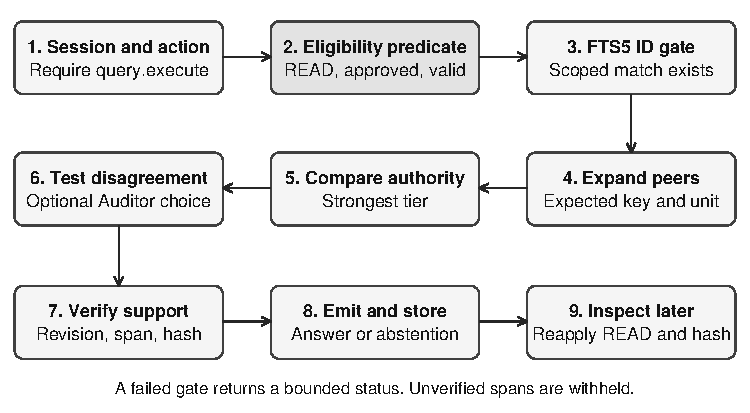
\includegraphics[width=0.89\linewidth,height=\textheight,keepaspectratio,alt={Strict
policy pipeline. The API combines authorization and reviewed eligibility
with the FTS identifier gate, expands peers, compares authority and
verifies evidence before returning a
status.}]{../figures/rendered/fig2.pdf}
\caption{Strict policy pipeline. The API combines authorization and
reviewed eligibility with the FTS identifier gate, expands peers,
compares authority and verifies evidence before returning a
status.}\label{fig:pipeline}
\end{figure}

Effective intervals are half-open: a policy remains applicable at its
start date but not at its end date. Thus, when one edition expires on
the day its successor takes effect, only the successor is eligible,
assuming the remaining conditions hold. Figure 3 shows why a revision
already issued by the query date can still be ineligible. Publication
and ingestion timestamps are stored separately and are not used as
effective-date cutoffs. This method answers which approved rule applies
to a date, not necessarily which rule an employee could have seen on
that historical date; reconstructing the latter would require
transaction-time history.

\begin{figure}
\centering
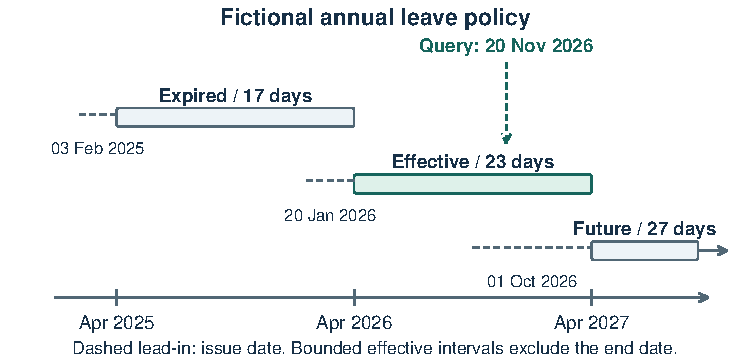
\includegraphics[width=0.89\linewidth,height=\textheight,keepaspectratio,alt={Fictional
leave policy timeline. On 20 November 2026 the April 2026 edition
applies although a future-effective edition has already been
issued.}]{../figures/rendered/fig3.pdf}
\caption{Fictional leave policy timeline. On 20 November 2026 the April
2026 edition applies although a future-effective edition has already
been issued.}\label{fig:timeline}
\end{figure}

\subsection{Authority, disagreement, and human
resolution}\label{authority-disagreement-and-human-resolution}

The admitted set must include the governing source kind, which is
operations policy for remote work and HR policy for the other three
topics. After confirming a single normalized claim key, the service
takes the highest numeric rank across the admitted set. When that tier
agrees on a value, the answer includes up to eight supporting spans. If
values differ, the service normally abstains and cites the conflicting
spans. If more than eight spans share the conflicting highest tier, it
abstains without a partial conflict citation set. A lower-tier
disagreement does not trigger conflict abstention. Figure 4 shows where
a recorded Auditor choice can resolve the exact conflict.

\begin{figure}
\centering
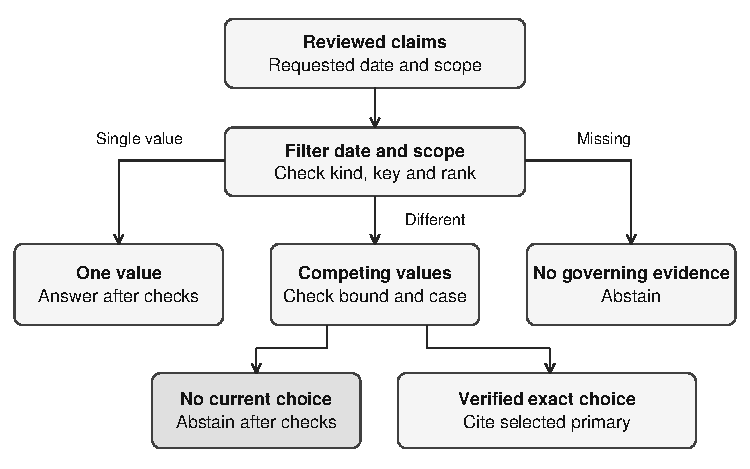
\includegraphics[width=0.89\linewidth,height=\textheight,keepaspectratio,alt={Authority
and conflict decision. Current competing values at the strongest tier
cause abstention unless an exact currently verified Auditor choice
applies.}]{../figures/rendered/fig4.pdf}
\caption{Authority and conflict decision. Current competing values at
the strongest tier cause abstention unless an exact currently verified
Auditor choice applies.}\label{fig:authority}
\end{figure}

Re-audit begins with an unresolved query owned by the requesting user
and still eligible for review. The backend recomputes the currently
authorized conflict and fingerprints the sorted evidence, including
claim keys, values, validity intervals, authority ranks, identifiers,
and hashes. An Auditor may select a primary source from precisely that
version set. Later questions can reuse the decision only when the
conflict fingerprint still matches and integrity checks succeed; the
answer identifies the human resolution. Undo restores abstention.
Changing a source, its authority, or the visible evidence set can
invalidate the earlier choice. Audited source grants may be issued to
the Auditor for the case, but this does not extend the Employee's READ
access.

\subsection{Citation verification and
provenance}\label{citation-verification-and-provenance}

For an evidence record with extracted text \(T\), character offsets
\(i,j\) and stored hex digest \(h\), fresh strict support checks require
\(T[i:j]\) to equal the quote and
\(\mathrm{SHA256}(\mathrm{UTF8}(T))=h\), with the hash expressed in
hexadecimal. The reviewed integer must appear without an adjacent digit.
These checks locate the reviewed span and detect text changes. They do
not independently establish entailment. The saved-answer path verifies
ownership, expiry, current READ on dependencies, policy and knowledge
revisions, and extracted-text digests. A revision change can invalidate
a saved result even when its cited text is unchanged. Figure 5 relates
the records used for these checks.

\begin{figure}
\centering
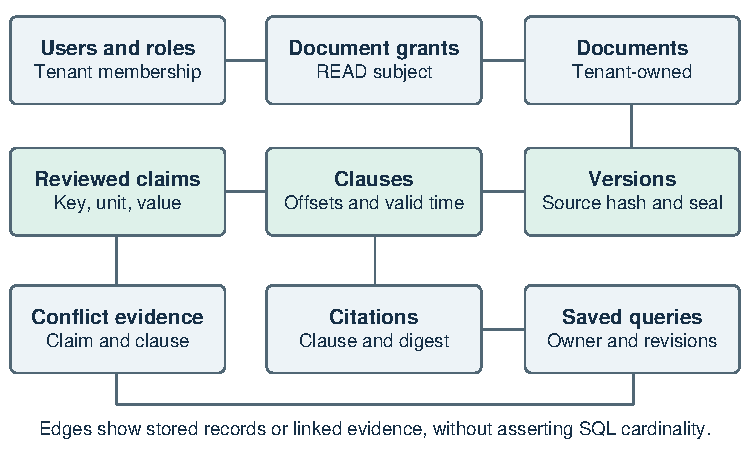
\includegraphics[width=0.89\linewidth,height=\textheight,keepaspectratio,alt={Evidence
relationships. User and role grants connect to documents and versions,
with approved clauses giving rise to claims, citations and conflict
evidence.}]{../figures/rendered/fig5.pdf}
\caption{Evidence relationships. User and role grants connect to
documents and versions, with approved clauses giving rise to claims,
citations and conflict evidence.}\label{fig:evidence}
\end{figure}

The system also stores an Ed25519 signature over a canonical upload
manifest \citep{rfc8032}. The manifest binds the tenant and version
identity to original-byte and extracted-text hashes and supplied
provenance fields. The integrity endpoint checks the configured key
identity, signature, stored metadata and independent hashes of the file
and extracted text. Re-audit resolution and reuse additionally check
signed source integrity. Ordinary strict answers rely on span, numeric
occurrence and extracted-text digest checks, so a routine citation
should not be interpreted as a fresh signature verification. A valid
seal establishes correspondence with the locally configured signer and
stored data. It cannot certify that a policy was authorized by an
external institution or that its content is correct.

\section{Implementation}\label{implementation}

We evaluated GitHub main commit
\href{https://github.com/NoirPrimordial7/cortex-ai/commit/dbbd2f293f312f3055db6beffc045e3e5b7ee62a}{dbbd2f2}.
React renders the question, date and scope controls, and evidence.
FastAPI and SQLAlchemy implement authenticated requests and
tenant-qualified queries over SQLite. FTS5 indexes policy clauses, and
Alembic manages schema revisions. A bounded child process extracts TXT,
text-bearing PDF and DOCX files under the local account. Original files
are stored privately. A reviewer marks the source span and normalized
numeric claim. Pending versions are excluded from strict retrieval.

The related-passage path uses BM25 over admitted lexical candidates and
optionally adds cosine-ranked vectors from the pinned local MiniLM
model. Reciprocal rank fusion combines the rankings using an offset of
60. This path can return passages when the service declines to give a
strict policy answer. It checks each exposed passage against its
extracted-text digest and offsets. The optional ranking does not change
the strict peer set. Personal leave records use a separate authorization
path outside the evaluation.

\section{Experimental Setup}\label{experimental-setup}

Figure 6 describes the two evaluation strata. The existing evaluator
seeds the development database and executes the repository's 12 cases.
Labels include status, selected clause IDs and eligible peer IDs.
Instrumentation observes admitted evidence in reasoning, selected
evidence in the answerer and a restricted marker in the response. The
evaluator opens the citation endpoint and recomputes the text hash. The
case count is distinct from frontend unit regressions, backend
regressions and actual browser flows.

\begin{figure}
\centering
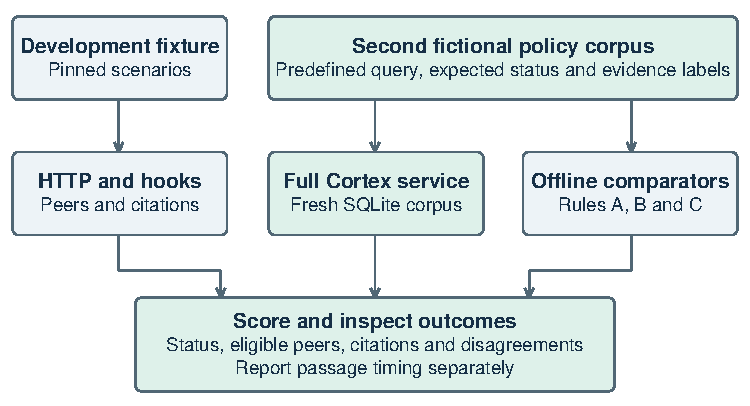
\includegraphics[width=0.89\linewidth,height=\textheight,keepaspectratio,alt={Evaluation
workflow. The development fixture and new fictional benchmark exercise
the pinned service, and offline comparator rules operate on the same
visible fictional policies.}]{../figures/rendered/fig6.pdf}
\caption{Evaluation workflow. The development fixture and new fictional
benchmark exercise the pinned service, and offline comparator rules
operate on the same visible fictional policies.}\label{fig:evaluation}
\end{figure}

The second fixture uses 12 short fictional policies and 16 questions
varying by date and scope. Before running the service, we specified the
expected answer or abstention, the eligible peer set, and the selected
citation set. A script then created an isolated database, removed
Employee access to the earlier seed documents, and introduced the new
policies through the application's ingestion, review, and distribution
endpoints. One policy remained pending, and another was approved but not
readable by the Employee. The labels and validity windows are included
with the reproducibility artifacts. Historical revisions, an exact
end-date transition, and simultaneous policies that agree on their
values serve as negative controls. Although two questions target a
conflict, both refer to the same underlying pair of policies.

All comparators operate over the same approved, visible policies and use
the same topic and population. Comparator A selects the latest-published
lexical match without enforcing effective dates or authority. B adds
valid-time filtering but still chooses a BM25 match and does not abstain
on disagreement. C further restricts B to the governing source kind,
which corresponds to the strongest tier in this particular fixture, but
still commits to a leading value. D is the full service. We ran A--C as
offline decision rules over the labeled policies and D through the
application's HTTP interface. The results compare their declared
outputs; they are not a causal isolation of individual components or of
production latency.

We record the identities and counts of eligible peers and selected
citations. For conflict detection we report true positives, false
positives and false negatives by question, and we give the number of
distinct disputes. Coverage is the share of queries that receive a
value. Citation checks re-fetch the source identified by the citation
and recompute its digest. Exposure checks for the second fixture track
two markers in the monitored stages and test direct reads. Warm
in-process requests include SQLite persistence and TestClient overhead.
The host ran Windows 11 on an Intel Core i7-13700F with Python 3.12.10,
SQLite 3.49.1, FastAPI 0.143.0 and SQLAlchemy 2.0.54. The new fixture's
full-route timing uses one annual-leave prompt, five preliminary
requests and 50 measured calls with the optional related-passage model
configured.

\section{Results}\label{results}

\subsection{Development fixture and software
verification}\label{development-fixture-and-software-verification}

The development fixture matched all 12 expected outcomes and recovered
all 15 labeled eligible policy-question pairs. All 10 citations matched
the stored spans and hashes. All five temporal cases and all four
expected abstentions passed. The service identified the single labeled
conflict without a false positive or a miss, and the restricted marker
was absent from the monitored stages and response payloads. The earlier
governance report records 97 backend tests, 39 frontend tests and 13
browser scenarios. At the pinned revision, 107 backend tests, including
local MiniLM inference, 44 frontend tests and six Chrome scenarios
passed. The backend run emitted one TestClient deprecation warning.
These software checks are separate from the fixture outcomes.

\subsection{New fictional policies and decision
rules}\label{new-fictional-policies-and-decision-rules}

The full service matched status, reason, value and selected sources on
16/16 questions. It returned all 19 eligible policy-question pairs with
no extra peers. Both positive questions were detected and none of the 14
negative questions was flagged. The two positive questions concern one
dispute. All five expected abstentions matched the labels and 11/16
questions received a value. All 16 returned citations passed exact span
and hash checks. Neither the pending-policy marker nor the
private-policy marker appeared in the monitored stages or responses.
Both direct reads by the Employee were denied. For 50 warm requests, the
development checker recorded a median of 11.670 ms and nearest-rank p95
of 15.887 ms. The separately configured full route recorded 28.721 ms
and 51.339 ms. The timings come from different fixtures and model
settings.

Table 1 summarizes the decision-rule comparison.

\begin{table}[!htbp]
\caption{Outcomes under different decision rules on 16 fictional queries. For A
to C a match means the expected value or no value. D also matches
status, reason and the selected evidence set.}\centering\small
\begin{tabular}{@{}>{\raggedright\arraybackslash}p{.24\linewidth}>{\raggedright\arraybackslash}p{.48\linewidth}>{\raggedright\arraybackslash}p{.17\linewidth}@{}}\toprule
\textbf{Variant} & \textbf{Decision rule} & \textbf{Matches} \\
\midrule
A & Lexical match, newest publication & 5/16 \\
B & Valid time, lexical selection & 14/16 \\
C & Governing authority, forced selection & 14/16 \\
D & Complete strict API & 16/16 \\
\bottomrule\end{tabular}
\end{table}

Three examples clarify the decision boundary. A leave edition published
in October is excluded from a November 2026 query because its effective
date lies in the future. During the remote-work overlap, both
conflicting records must be considered; at the exact end of that
overlap, the remaining policy governs. Simultaneous notice clauses with
identical values do not create a conflict. Authority filtering adds no
matches beyond B in this particular fixture because B's lexical ranking
already selects the governing source in its lower-tier example.

\subsection{Optional passage ranking and
latency}\label{optional-passage-ranking-and-latency}

Across four exploratory related-passage prompts, the designated policy
appeared once with hybrid ranking and zero times with lexical-only
ranking. The hybrid path found the remote-work policy for a
telecommuting paraphrase and also returned unrelated passages. Because
the service removes strict citations from the related list, the observed
count combines retrieval and deduplication. The strict decision is
unchanged by the optional ranking. For the paraphrase, each condition
used five preliminary requests and 30 measured warm requests. The
lexical-only median and nearest-rank p95 were 10.329 ms and 11.692 ms.
With the CPU encoder enabled, they were 27.763 ms and 45.733 ms. Both
conditions used the same route and data and ran sequentially. Memory use
and scaling remain unmeasured.

\section{Discussion}\label{discussion}

Peer expansion helps expose an incompatible claim even when that claim
is a weaker lexical match. It cannot help, however, if no eligible
document passes the initial full-text gate. Incorrect review metadata
may also exclude a relevant peer before comparison. Conversely, a
high-authority source can settle the final answer while leaving a
meaningful lower-tier inconsistency out of the employee-facing response.
A separate reviewer workflow would be needed to surface those
discrepancies without changing what the employee is permitted to see.

Document grants affect the answer itself, not only which citations
appear. Two users asking about the same date may receive different
outcomes because they are allowed to see different policies. If one
source is restricted, even announcing that a hidden conflict exists
could disclose information. Organizations that need a common explanation
across roles would therefore have to publish a separately authorized
summary written or approved by a reviewer.

Exact-span checking establishes that a citation matches the stored
extracted text and its digest. The signed manifest, by contrast, ties
the original and extracted artifacts to the configured signer. Neither
check decides which policy should prevail or whether its wording has
been interpreted correctly. Both depend on reliable document collection,
review, and custody.

\section{Threats to Validity and
Limitations}\label{threats-to-validity-and-limitations}

The study uses two deliberately constructed policy collections rather
than a sample drawn from enterprise records. Independent reviewers have
not adjudicated the new labels, and the two positive conflict questions
concern one disagreement. Reusing documents across questions also
reduces the amount of independent evidence in the results. Accordingly,
the outcomes describe these scenarios; they do not show superiority over
tuned temporal search systems or commercial enterprise retrieval
products.

Reviewed metadata is itself a source of error: an incorrect effective
interval can make an otherwise sound decision wrong. READ grants apply
at document level and cannot express exceptions hidden in particular
sections. Cortex does not infer arbitrary natural-language
contradictions or automatically reconcile amendments, nor does its
clause model cover every condition found in long legal or HR documents.
Signed provenance cannot help if an attacker controls both the signer
and the trusted storage. Finally, canary checks and denied reads cover
observed application paths, not every possible timing,
indirect-disclosure, or copied-data channel.

The timing measurements come from repeated short requests against a
small SQLite database on one host. They do not characterize large
corpora, concurrent users, memory pressure, or distributed operation.
Likewise, browser regression tests confirm the exercised behavior and
layouts, not usability or reliability under every device and network
condition.

\section{Conclusion and Future Work}\label{conclusion-and-future-work}

Cortex AI answers four policy topics using current authorization,
reviewed effective dates, authority ranks, conflict abstention, and
version-bound citations. A specific conflict can be resolved through a
recorded, verifiable human decision. The controlled fictional
evaluations show that these mechanisms behave as intended in the cases
tested, while leaving real-enterprise generalization open.

The next evaluation should use larger, independently annotated
multi-version documents and stronger temporal baselines, with latency
and memory measured as the corpus grows. Additional integrity
experiments should test reviewer mistakes, versioned metadata,
signing-key lifecycle, and information disclosed through the audit
workflow.

\subsection{Reproducibility and
disclosure}\label{reproducibility-and-disclosure}

The reviewed inputs are fictional. The manuscript package includes
corpus labels, baseline code, a pinned implementation identifier, run
outputs and figure sources. Reproduction uses fictional records and
local test keys. Codex assisted with source verification, benchmark and
diagram code, drafting and editing. The final disclosure wording and
authorship details remain subject to author approval.
\bibliographystyle{splncs04}
\bibliography{../bibliography/references}
\end{document}
